\documentclass{beamer}
\usetheme{tokitex}

\usepackage{graphics}
\usepackage{multirow}
\usepackage{tabto}

\usepackage[english,bahasa]{babel}
\newtranslation[to=bahasa]{Section}{Bagian}
\newtranslation[to=bahasa]{Subsection}{Subbagian}

\usepackage{listings}
\usepackage{color}

\definecolor{dkgreen}{rgb}{0,0.6,0}
\definecolor{gray}{rgb}{0.5,0.5,0.5}
\definecolor{mauve}{rgb}{0.58,0,0.82}

\lstset{frame=tb,
  language=pascal,
  aboveskip=3mm,
  belowskip=3mm,
  showstringspaces=false,
  columns=flexible,
  basicstyle={\small\ttfamily},
  numbers=none,
  numberstyle=\tiny\color{gray},
  keywordstyle=\color{blue},
  commentstyle=\color{dkgreen},
  stringstyle=\color{mauve},
  breaklines=true,
  breakatwhitespace=true,
  tabsize=3
}

\title{Halo Dunia}
\author{Tim Olimpiade Komputer Indonesia}

\begin{document}

\begin{frame}
\titlepage
\end{frame}

\begin{frame}
\frametitle{Pendahuluan}
Melalui dokumen ini, kalian akan:
\begin{itemize}
	\item Mengenal program, pemrograman, dan bahasa pemrograman
	\item Memahami bagaimana program dieksekusi
	\item Mengenal kompilator
	\item Mengenal bahasa Pascal
	\item Melakukan instalasi perangkat lunak yang dibutuhkan untuk pemrograman Pascal
\end{itemize}
\end{frame}

\section{Pengenalan Pemrograman}
\frame{\sectionpage}

\begin{frame}
\frametitle{Apa itu Program?}
\begin{block}{Program}
	Serangkaian instruksi yang dieksekusi oleh mesin untuk mencapai suatu tujuan tertentu.
\end{block}
\begin{itemize}
	\item Biasanya, program dapat menerima masukan, memprosesnya, dan menghasilkan suatu keluaran.
	\item Contoh: program penerjemah bahasa menerima berkas dalam suatu bahasa sebagai masukan, menerjemahkannya, lalu menghasilkan keluaran berupa hasil terjemahannya.
\end{itemize}
\end{frame}

\begin{frame}
\frametitle{Pemrograman dan Bahasa Pemrograman}
\begin{itemize}
	\item Pemrograman adalah aktivitas menulis program.
	\item Program ditulis dengan bahasa pemrograman, sehingga mesin atau komputer dapat mengerti apa yang yang diinstruksikan.
	\item Contoh bahasa pemrograman yang populer adalah C, C++, Pascal, Java, dan Python. 
	\item Pada pembelajaran ini, kita akan menggunakan bahasa Pascal.
\end{itemize}
\end{frame}

\begin{frame}
\frametitle{Bagaimana Komputer Menjalankan Program?}
\begin{itemize}
	\item Pada masa lalu, komputer diprogram dengan menuliskan sederetan instruksi dalam bahasa Assembly.
	\item Bahasa Assembly mudah dimengerti oleh mesin, sehingga mudah untuk dieksekusi. Oleh karena itu, Bahasa Assembly termasuk dalam bahasa pemrograman tingkat rendah (dekat dengan mesin).
	\item Meskipun begitu, membaca dan mengerti alur program Assembly cukup sulit bagi manusia.
\end{itemize}
\end{frame}

\begin{frame}
\frametitle{Bagaimana Komputer Menjalankan Program? (lanj.)}
\begin{itemize}
	\item Pada tahun 1960-an, mulai diciptakan bahasa pemrograman tingkat tinggi.
	\item Bahasa-bahasa ini lebih mudah dimengerti manusia karena menggunakan frase bahasa sehari-hari, seperti "jika ... maka ...", "lakukan ... hingga tercapai ...", dan sebagainya.
	\item Sayangnya, bahasa pemrograman tingkat tinggi tidak bisa dimengerti secara langsung oleh mesin. Perlu ada penerjemahan bahasa pemrograman tingkat tinggi ke tingkat rendah, sehingga mesin dapat mengerti instruksi-instruksi yang diberikan.
	\item Penerjemahan ini biasa dilakukan oleh program yang berperan sebagai kompilator, intepreter, atau keduanya. Dalam hal ini kita hanya akan membahas tentang kompilator.
\end{itemize}
\end{frame}

\begin{frame}
\frametitle{Kompilator}
\begin{itemize}
	\item Merupakan program komputer yang dapat menerjemahkan bahasa pemrograman tingkat tinggi ke bahasa mesin.
	\item Hasil terjemahan ini yang nantinya dapat dimengerti oleh mesin, sehingga dapat dieksekusi oleh komputer.
	\item Aktivitas menerjemahkan ini disebut dengan kompilasi.
	\item Siklus kerja jika kita menggunakan kompilator adalah: tulis program $\rightarrow$ kompilasi $\rightarrow$ eksekusi.
\end{itemize}
\end{frame}

\begin{frame}
\frametitle{Mengapa Pascal?}
\begin{itemize}
	\item Mudah dibaca dan dikelola dibandingkan dengan bahasa C/C++.
	\item Mudah untuk melakukan kompilasi.
	\item Kompilasi berjalan dengan cepat.
\end{itemize}
\end{frame}

\begin{frame}
\frametitle{Tentang Free Pascal}
\begin{itemize}
	\item Merupakan salah satu kompilator Pascal yang populer.
	\item Program kompilator Free Pascal beserta dokumentasinya tersedia gratis.
	\item Free Pascal merupakan kompilator resmi yang dipakai pada IOI (\textit{International Olympiad in Informatics}/Olimpiade Informatika Internasional).
	\item Free Pascal memenuhi standar dalam bahasa Pascal.
\end{itemize}
\end{frame}

\section{Petunjuk Mempersiapkan Lingkungan Belajar}
\frame{\sectionpage}

\begin{frame}
\frametitle{Instalasi Free Pascal (Windows)}
\begin{itemize}
	\item Seluruh petunjuk instalasi yang akan diberikan ini akan dilakukan pada sistem operasi Windows 7.
	\item Proses instalasi berikut akan menghasilkan dua hal muncul pada komputer kalian, yaitu:
	\begin{itemize}
		\item Kompilator Free Pascal.
		\item IDE (\textit{Integrated Development Environment}) bawaan dari Free Pascal. IDE ini bisa dianggap sebagai sebuah lingkungan tempat kalian memprogram nantinya.
	\end{itemize}
	\item Buka \textit{browser} kalian dan kunjungi http://www.freepascal.org/download.var
	\item Unduh sesuai dengan arsitektur prosesor komputer kalian, misalnya intel dan Windows 32 bit
\end{itemize}
\end{frame}

\begin{frame}
\frametitle{Instalasi Free Pascal (Windows) (lanj.)}
\begin{itemize}
	\item Berikut ini adalah tampilan dari http://www.freepascal.org/download.var
\end{itemize}
\begin{figure}
	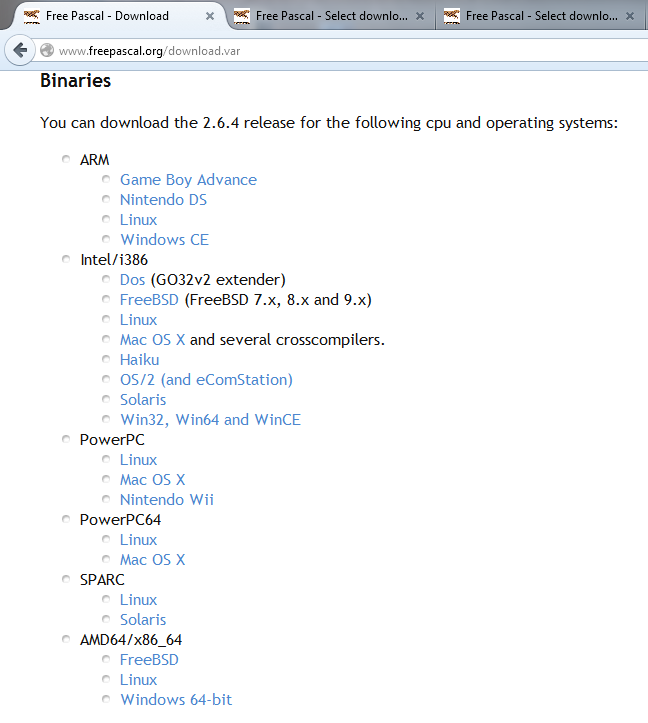
\includegraphics[width=6cm]{asset/dl_list1.PNG}
\end{figure}
\end{frame}

\begin{frame}
\frametitle{Instalasi Free Pascal (Windows) (lanj.)}
\begin{itemize}
	\item Setelah selesai mengunduh, jalankan \textit{installer} Free Pascal yang baru saja diunduh.
	\begin{figure}
		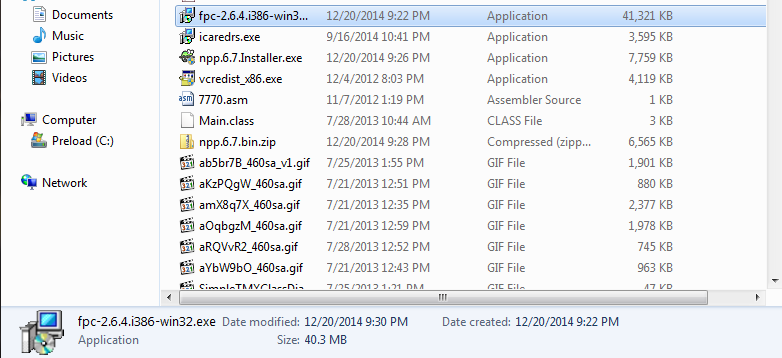
\includegraphics[width=9cm]{asset/fpc_1.PNG}
	\end{figure}
\end{itemize}
\end{frame}

\begin{frame}
\frametitle{Instalasi Free Pascal (Windows) (lanj.)}
\begin{itemize}
	\item Akan muncul tampilan sebagai berikut:
	\begin{figure}
		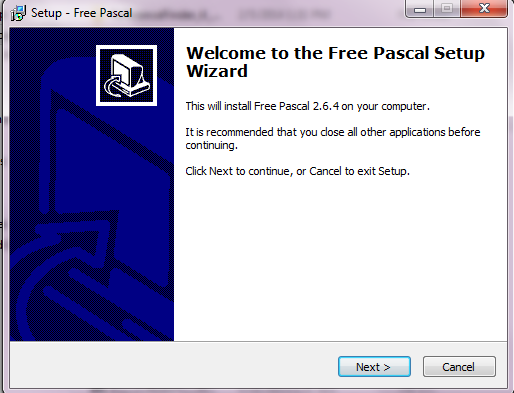
\includegraphics[width=4cm]{asset/fpc_2.PNG}
	\end{figure}
	\item Pilih \textit{next}, terus hingga sampai pada tampilan berikut:
	\begin{figure}
		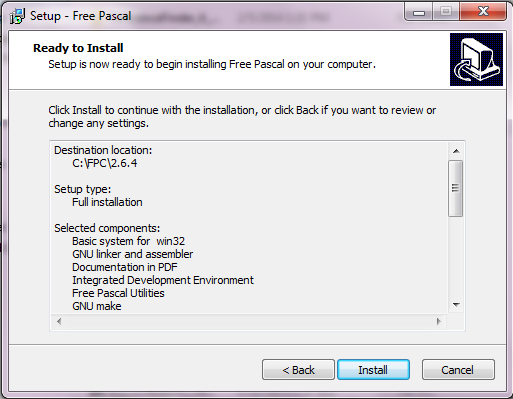
\includegraphics[width=4cm]{asset/fpc_7.PNG}
	\end{figure}
\end{itemize}
\end{frame}

\begin{frame}
\frametitle{Instalasi Free Pascal (Windows) (lanj.)}
\begin{itemize}
	\item Pilih \textit{install} dan proses instalasi akan segera berjalan.
	\item Jika sudah selesai, pilih \textit{next} dan \textit{finish}.
	\begin{figure}
		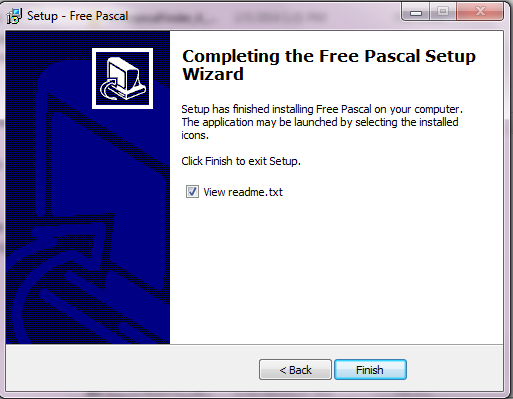
\includegraphics[width=6cm]{asset/fpc_10.PNG}
	\end{figure}
\end{itemize}
\end{frame}

\begin{frame}
\frametitle{Instalasi Free Pascal (Windows) (lanj.)}
\begin{itemize}
	\item Jika kalian menjalankan program Free Pascal, tampilan berikut akan muncul:
	\begin{figure}
		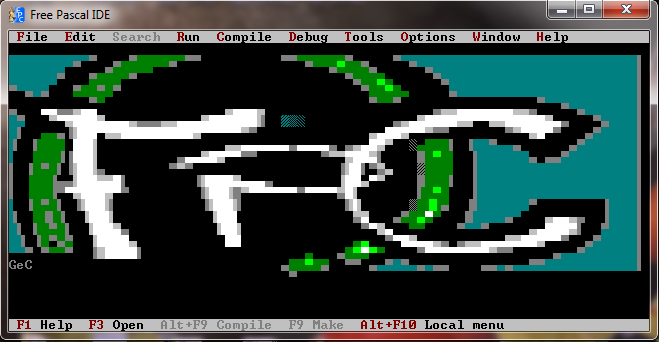
\includegraphics[width=9cm]{asset/fpc_11.PNG}
	\end{figure}
\end{itemize}
\end{frame}

\begin{frame}
\frametitle{Lingkungan Pemrograman}
\begin{itemize}
	\item Sejauh ini, memprogram dengan Free Pascal sudah bisa dilakukan. 
	\item Namun, memprogram langsung dari IDE Free Pascal biasanya kurang nyaman; banyak keterbatasannya meskipun ada beberapa keuntungannya (seperti fitur \textit{debugging}).
	\item Untuk itu, kami akan memperkenalkan penggunaan \textit{text editor} yang cukup populer, yaitu Notepad++.
	\item Kalian akan menulis kode di Notepad++, lalu melakukan kompilasi dan eksekusi program di \textit{command line}. Praktik sejenis ini merupakan kebiasaan dari para peserta IOI, dan ada baiknya dilatih sejak awal kalian belajar memprogram \text{:)}
\end{itemize}
\end{frame}

\begin{frame}
\frametitle{Perkenalan Notepad++}
\begin{itemize}
	\item Notepad++ merupakan perangkat lunak pengolah teks yang sifatnya gratis dan berjalan di sistem operasi Windows.
	\item Sesuai dengan namanya, kalian bisa menganggap bahwa Notepad++ merupakan versi "plus-plus" dari Notepad, yang mana membuatnya lebih canggih dari Notepad.
	\item Kalian dapat menggunakan Notepad++ untuk berbagai keperluan, seperti menulis program dalam bahasa C, C++, atau Pascal.
\end{itemize}
\end{frame}

\begin{frame}
\frametitle{Instalasi Notepad++ (Windows)}
\begin{itemize}
	\item Buka kembali \textit{browser} kalian, dan kunjungi http://notepad-plus-plus.org/download/v6.7.html
	\begin{figure}
		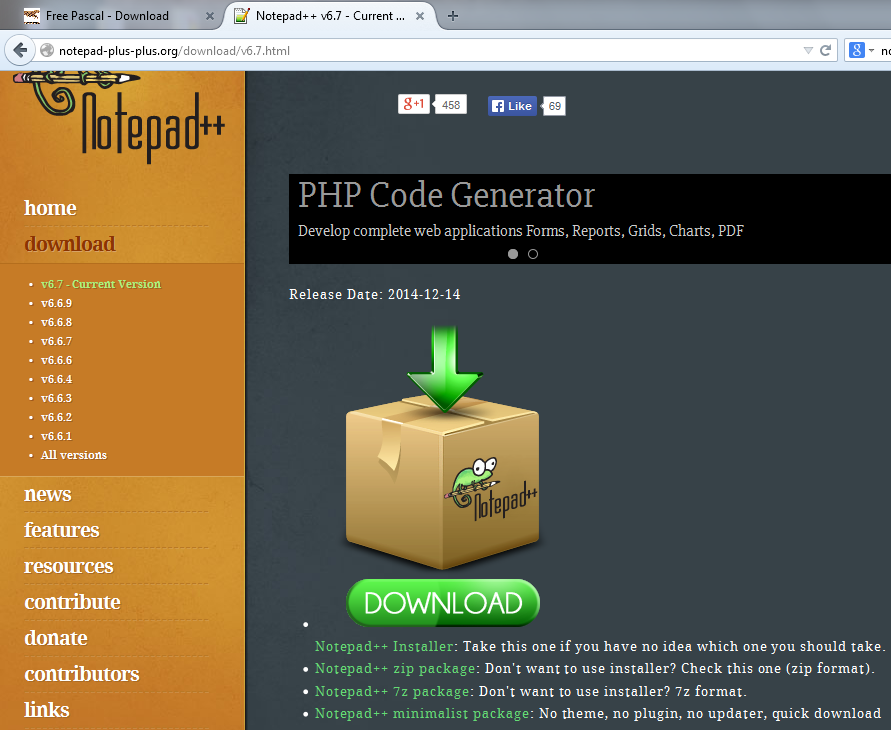
\includegraphics[width=6cm]{asset/npp_1.PNG}
	\end{figure}
	\item Unduh \textit{installer} Notepad++ dengan memilih \textit{Notepad++ Installer} di bagian bawah tombol \textit{download}.
\end{itemize}
\end{frame}

\begin{frame}
\frametitle{Instalasi Notepad++ (Windows) (lanj.)}
\begin{itemize}
	\item Jalankan \textit{installer} Notepad++ yang baru kalian unduh.
	\item Akan muncul tampilan sebagai berikut:
	\begin{figure}
		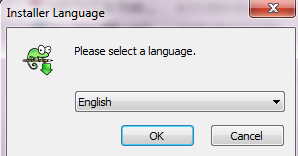
\includegraphics[width=3cm]{asset/npp_3.PNG}
	\end{figure}
	\item Pilih \textit{ok}, lalu \textit{next} sampai muncul tampilan berikut:
	\begin{figure}
		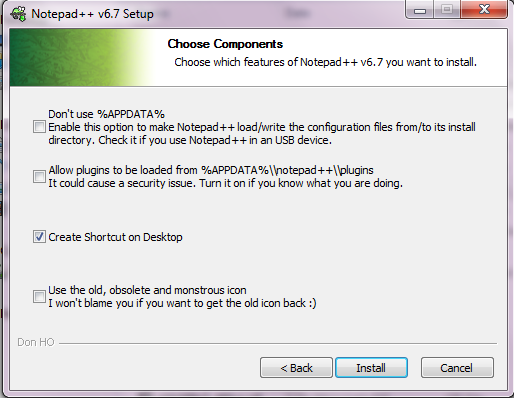
\includegraphics[width=5cm]{asset/npp_7.PNG}
	\end{figure}
\end{itemize}
\end{frame}

\begin{frame}
\frametitle{Instalasi Notepad++ (Windows) (lanj.)}
\begin{itemize}
	\item Pilih \textit{install}, dan tunggu sampai proses instalasi selesai.
	\item Setelah muncul tampilan berikut, pilih \textit{finish}.
	\begin{figure}
		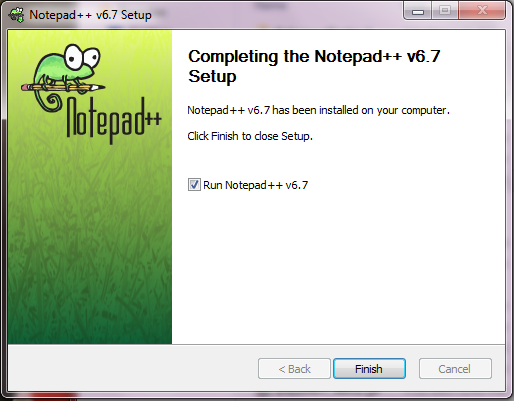
\includegraphics[width=5cm]{asset/npp_9.PNG}
	\end{figure}
\end{itemize}
\end{frame}

\begin{frame}[fragile]
\frametitle{Menulis Program Pascal Sederhana}
\begin{itemize}
	\item Ketikkan program berikut pada Notepad++, lalu simpan dengan nama halo.pas di suatu direktori, misalnya di Desktop.
\end{itemize}
\begin{lstlisting}
begin
    writeln('Halo Dunia!');
end.
\end{lstlisting}
\end{frame}

\begin{frame}
\frametitle{Kompilasi Program Pascal}
\begin{itemize}
	\item Buka cmd, yang bisa dilakukan dengan cara menekan tombol winkey+r, lalu isikan "cmd" pada kotak dialog yang muncul, dan tekan enter.
	\item Pergi ke direktori tempat halo.pas disimpan, gunakan perintah "cd .." untuk mundur ke direktori \textit{parent} dan "cd $<$nama folder$>$" untuk maju ke direktori $<$nama folder$>$.
	\begin{figure}
		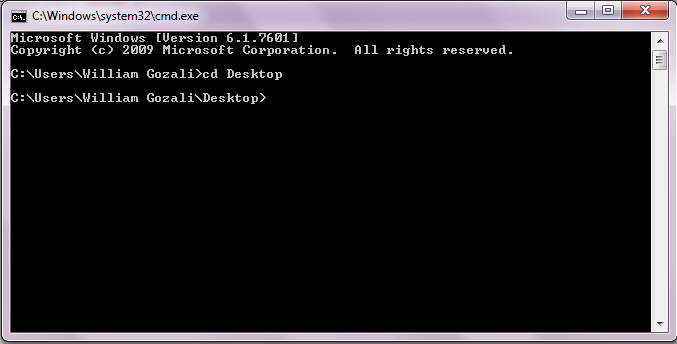
\includegraphics[width=7cm]{asset/hello_2.PNG}
	\end{figure}
\end{itemize}
\end{frame}

\begin{frame}
\frametitle{Kompilasi Program Pascal (lanj.)}
\begin{itemize}
	\item Ketikkan "fpc halo.pas" pada cmd.
	\item Perhatikan bahwa mungkin akan muncul pesan kesalahan seperti berikut ini:
	\begin{figure}
		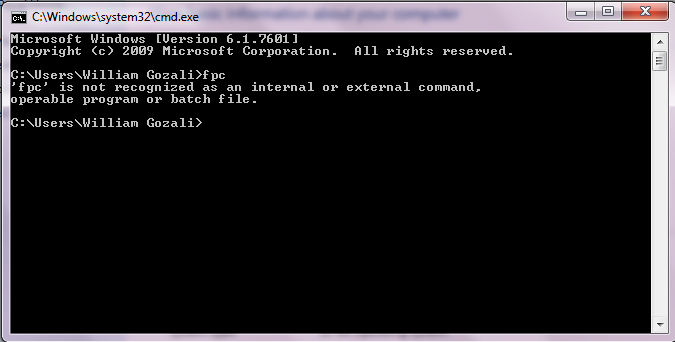
\includegraphics[width=7cm]{asset/cmd_0.PNG}
	\end{figure}
	\item Jika ini terjadi, artinya perlu pengaturan \textit{path} FPC terlebih dahulu.
\end{itemize}
\end{frame}

\begin{frame}[fragile]
\frametitle{Kompilasi Program Pascal (lanj.)}
\begin{itemize}
	\item Ketikkan "fpc halo.pas" pada cmd.
	\item Perhatikan bahwa mungkin akan muncul pesan kesalahan seperti berikut ini:
\end{itemize}
\begin{quote}
'fpc' is not recognized as an internal or external command, operable program or batch file.
\end{quote}
\begin{itemize}
	\item Jika ini terjadi, artinya perlu pengaturan \textit{path} FPC pada \textit{environment variable} terlebih dahulu.
\end{itemize}
\end{frame}

\begin{frame}
\frametitle{Pengaturan \textit{environment variable}}
\begin{itemize}
	\item Klik kanan pada "my computer", lalu pilih \textit{properties}. Akan muncul tampilan sebagai berikut:
	\begin{figure}
		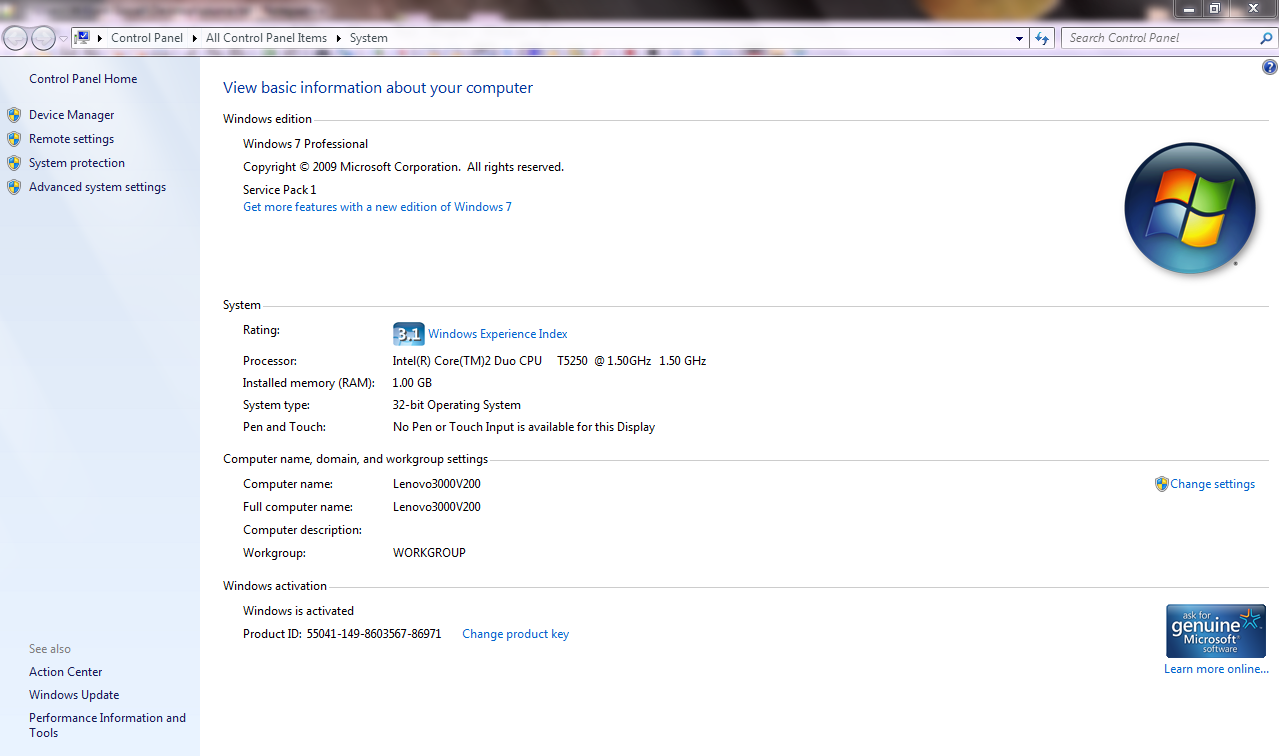
\includegraphics[width=10cm]{asset/path_1.PNG}
	\end{figure}
	\item Pilih \textit{advanced system settings} di bagian kiri.
\end{itemize}
\end{frame}

\begin{frame}
\frametitle{Pengaturan \textit{environment variable} (lanj.)}
\begin{itemize}
	\item Pilih tab \textit{advance}, lalu tekan tombol \textit{environment variable}.
	\begin{figure}
		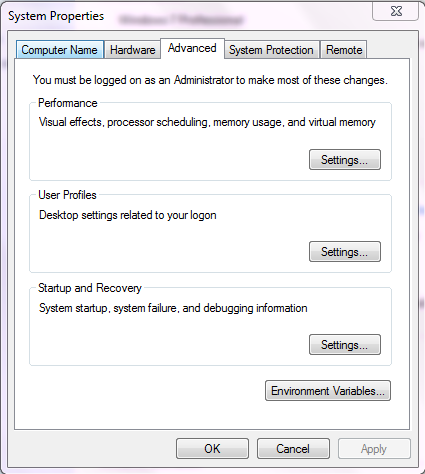
\includegraphics[width=6cm]{asset/path_2.PNG}
	\end{figure}
\end{itemize}
\end{frame}

\begin{frame}
\frametitle{Pengaturan \textit{environment variable} (lanj.)}
\begin{itemize}
	\item Kemudian akan muncul tampilan sebagai berikut:
	\begin{figure}
		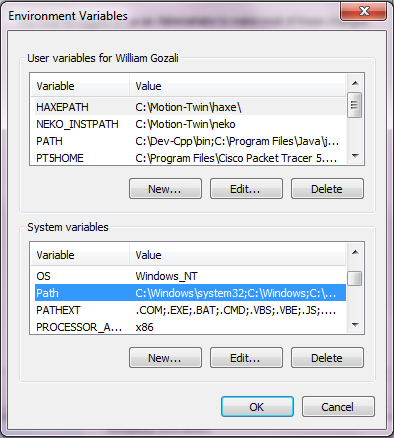
\includegraphics[width=6cm]{asset/path_3.PNG}
	\end{figure}
\end{itemize}
\end{frame}

\begin{frame}
\frametitle{Pengaturan \textit{environment variable} (lanj.)}
\begin{itemize}
	\item Pada bagian \textit{system variables}, pilih \textit{Path} lalu tekan tombol \textit{edit}. Jika kalian tidak bisa menemukannya, maka tekan tombol \textit{new}.
	\item Isikan direktori tempat Free Pascal kalian disimpan. Pastikan direktori yang kalian isi lengkap, contohnya:
	\begin{figure}
		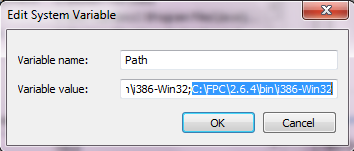
\includegraphics[width=6cm]{asset/path_4.PNG}
	\end{figure}
	\item Tekan \textit{ok} hingga seluruh kotak dialog tertutup.
\end{itemize}
\end{frame}

\begin{frame}
\frametitle{Pengaturan \textit{environment variable} (lanj.)}
\begin{itemize}
	\item Tutup cmd yang telah terbuka, lalu buka kembali.
	\item Pergi ke direktori tempat halo.pas disimpan dan ketikkan "fpc halo.pas".
	\item Pastikan muncul tulisan seperti berikut:
	\begin{figure}
		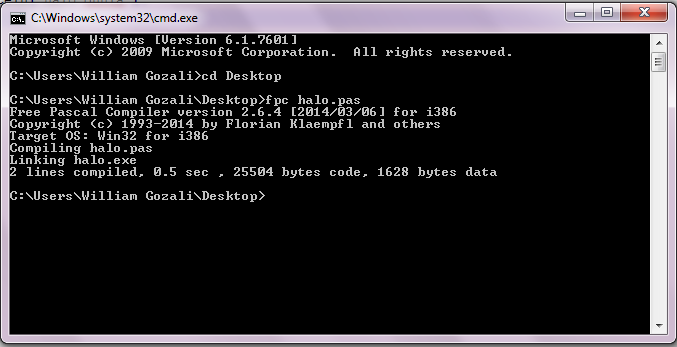
\includegraphics[width=9cm]{asset/hello_3.PNG}
	\end{figure}
	\item Selamat! Kompilasi berhasil dilaksanakan!
\end{itemize}
\end{frame}

\begin{frame}
\frametitle{Kompilasi Program Pascal (lanj.)}
\begin{itemize}
	\item Ketikkan "halo" pada cmd, yang artinya menjalankan program "halo.pas" yang sudah dikompilasi.
	\item Pastikan tulisan "halo dunia" tercetak di cmd!
	\begin{figure}
		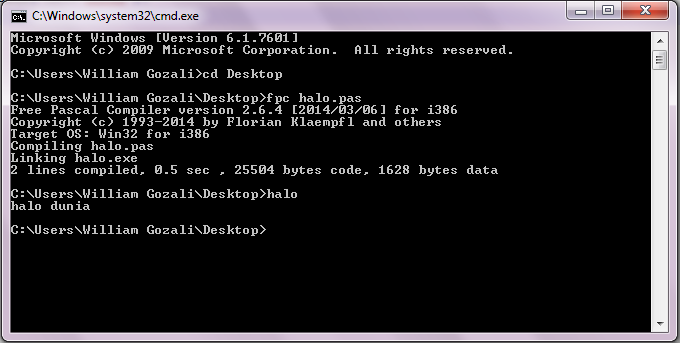
\includegraphics[width=9cm]{asset/hello_4.PNG}
	\end{figure}
	\item Selamat! Kalian berhasil menulis dan menjalankan program Pascal!
\end{itemize}
\end{frame}

\begin{frame}
\frametitle{Selanjutnya...}
\begin{itemize}
	\item Pengenalan variabel dan tipe data.
	\item Pengenalan baca masukan dan cetak keluaran.
	\item Pemrograman Pascal sederhana.
\end{itemize}
\end{frame}

\end{document}